\section{单纯同调与奇异同调之间的同构}
\sourcepage{221--222}
本节证明：若 $K$ 是单纯复形，则 $K$ 的单纯同调群同构于 $|K|$ 的奇异同调群。这个同构还与诱导同态及边缘同态 $\partial_*$ 可交换，所以它是两种同调理论之间的同构。

证明使用第 1.14 节的有序链复形 $\{C'_p(K),\partial'\}$。那里已证明，有序同调群同构于通常的有向单纯同调群。本节再证明它同构于 $|K|$ 的奇异同调群，从而在多面体上把单纯同调与奇异同调联系起来。

回忆有序 $p$ 维单形是顶点的 $(p+1)$ 元组 $(v_0,\ldots,v_p)$，其中顶点可重复，但必须张成 $K$ 中的一个单形。群 $C'_p(K)$ 以这些元组为自由基，且
\[
\partial'(v_0,\ldots,v_p)=\sum_{i=0}^p(-1)^i(v_0,\ldots,\widehat v_i,\ldots,v_p),\qquad \epsilon'(v)=1.
\]

\entry{定义}{4.7.1}定义 $\theta:C'_p(K)\to S_p(|K|)$，令
\[
\theta((v_0,\ldots,v_p))=\ell(v_0,\ldots,v_p).
\]
即把有序单形映为将 $\epsilon_i$ 映到 $v_i$ 的线性奇异单形。由定义，$\theta$ 是保持增广的链映射，并与包含映射可交换。因此对任何子复形 $K_0$，它诱导相对链映射
\[
\theta:C'_p(K,K_0)\to S_p(|K|,|K_0|).
\]
为证明 $\theta_*$ 是同构，先给出一个引理。

\entry{引理}{4.7.2}设 $\psi:C\to C'$ 是增广链复形的链映射。则 $\psi_*$ 在约化同调上为同构，当且仅当它在普通同调上为同构。

\textbf{证明：}回忆 $H_0(C)\cong\widetilde H_0(C)\oplus\Z$ 的证明（第 1.8 节习题）。考虑交换图
\[
\begin{array}{ccccccccc}
0&\to&\ker\epsilon&\to&C_0&\xrightarrow{\epsilon}&\Z&\to&0\\
&&\downarrow\scriptstyle\psi&&\downarrow\scriptstyle\psi&&\downarrow\scriptstyle=&&\\
0&\to&\ker\epsilon'&\to&C'_0&\xrightarrow{\epsilon'}&\Z&\to&0.
\end{array}
\]
取 $j:\Z\to C_0$，使 $\epsilon\circ j=\operatorname{id}_{\Z}$，并令 $j'=\psi j$。\translatornote{原书把分裂条件写为 $j\circ\epsilon$ 是恒等映射；正确的条件为 $\epsilon\circ j=\operatorname{id}_{\Z}$。}两个短正合列分别由 $j,j'$ 分裂，故
\[
C_0=\ker\epsilon\oplus\operatorname{im}j,\qquad C'_0=\ker\epsilon'\oplus\operatorname{im}j'.
\]
映射 $\psi$ 把 $\operatorname{im}j$ 同构地映到 $\operatorname{im}j'$，而
\[
H_0(C)\cong\frac{\ker\epsilon}{\partial C_1}\oplus\operatorname{im}j,\qquad
H_0(C')\cong\frac{\ker\epsilon'}{\partial'C'_1}\oplus\operatorname{im}j'.
\]
因此普通零维同调上的同态为同构，恰当且仅当约化零维同调上的同态为同构。正维数中两种同调本来相同。\hfill$\square$

\entry{引理}{4.7.3}若 $K_0$ 是 $K$ 的子复形，则对每个 $p$，$\theta$ 诱导同构
\begin{enumerate}[label=(\arabic*)]
\item $\theta_*:\widetilde H_p(\mathcal C'(K))\to\widetilde H_p(|K|)$；
\item $\theta_*:H_p(\mathcal C'(K))\to H_p(|K|)$；
\item $\theta_*:H_p(\mathcal C'(K,K_0))\to H_p(|K|,|K_0|)$。
\end{enumerate}

\sourcepage{223}
\textbf{证明：}可设 $K_0\ne K$，否则 (3) 显然。

\textbf{步骤 1：}先对有限复形按单形个数 $n$ 归纳。若 $n=1$，$K$ 只有一个顶点 $v$。每一维只有一个有序单形 $(v,\ldots,v)$，也只有一个奇异单形 $T:\Delta_p\to\{v\}$，且 $\theta(v,\ldots,v)=T$。所以 $\theta$ 在链的层次上就是同构，三个结论都成立。

设对少于 $n$ 个单形的复形结论成立，而 $K$ 有 $n$ 个单形。只需证明 (1)：由引理 4.7.2 可得 (2)；对子复形 $K_0$ 应用归纳假设，再由长正合列及 Steenrod 五引理可得 (3)。

取 $K$ 中维数最大的单形 $\sigma$。它不是其他单形的真面，故删去 $\sigma$ 后其余单形组成有 $n-1$ 个单形的子复形 $K_1$。令 $\Sigma$ 由 $\sigma$ 及其所有面组成，$\Bd\Sigma$ 由其真面组成。考虑交换图
\[
\begin{array}{ccc}
\widetilde H_p(\mathcal C'(K))&\xrightarrow{\theta_*}&\widetilde H_p(|K|)\\
\downarrow\scriptstyle i_*&&\downarrow\scriptstyle i_*\\
H_p(\mathcal C'(K,\Sigma))&\xrightarrow{\theta_*}&H_p(|K|,\sigma)\\
\uparrow\scriptstyle j_*&&\uparrow\scriptstyle j_*\\
H_p(\mathcal C'(K_1,\Bd\Sigma))&\xrightarrow{\theta_*}&H_p(|K_1|,\Bd\sigma).
\end{array}
\]
其中 $i,j$ 是包含映射；若 $\dim\sigma=0$，两个边缘均为空。由归纳假设，底行同态是同构。下面证明各竖直同态为同构，于是顶行也是同构。

由于 $\sigma$ 的奇异同调无环，空间偶 $(|K|,\sigma)$ 的长正合列说明右侧 $i_*$ 为同构。有序同调中，$\Sigma$ 由引理 1.14.14 无环，同样说明左侧 $i_*$ 为同构。

左侧 $j_*$ 由链层次的同构诱导：包含映射 $\mathcal C'(K_1)\to\mathcal C'(K)/\mathcal C'(\Sigma)$ 满射，其核恰为由 $K_1\cap\Sigma=\Bd\Sigma$ 承载的链。实际上，这正是一个切除映射。

\sourcepage{224}
但不能直接把奇异同调中的 $j$ 也看作切除映射。其定义域由删去开单形 $U=\Int\sigma$ 得到，然而 $\overline U=\sigma$，删去的集合太大，不能应用定理 4.4.10。我们改为只删去重心 $\widehat\sigma$。把 $j$ 分解为包含映射
\[
(|K_1|,\Bd\sigma)\xrightarrow{k}(|K|\setminus\{\widehat\sigma\},\sigma\setminus\{\widehat\sigma\})
\xrightarrow{\ell}(|K|,\sigma).
\]
单点 $\{\widehat\sigma\}$ 闭且包含于 $\sigma$ 在 $|K|$ 中的内部，故 $\ell$ 是合法的切除映射，$\ell_*$ 为同构。这里开单形 $\Int\sigma=|K|\setminus|K_1|$ 是开集，因为 $|K_1|$ 闭。\translatornote{原书进一步说 $\sigma$ 的点集拓扑内部等于其开单形，这一般不成立；本论证只需后者是包含重心的开邻域。}

若 $\dim\sigma=0$，则 $k$ 为恒等映射。若 $\dim\sigma>0$，$\Bd\sigma$ 是 $\sigma\setminus\{\widehat\sigma\}$ 的形变收缩核。令形变在 $|K_1|$ 上为恒等，即将它延拓为 $|K|\setminus\{\widehat\sigma\}$ 到 $|K_1|$ 的形变收缩，见图 4.7.1。由定理 4.3.9，$k_*$ 为同构，因此 $j_*=\ell_*k_*$ 为同构。
\begin{center}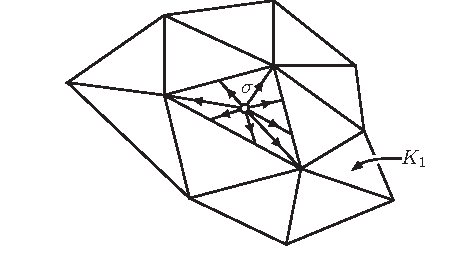
\includegraphics[width=.65\textwidth]{figures/4-7-1.pdf}\\图 4.7.1\end{center}

\textbf{步骤 2：}现在处理任意复形。仍只需证明 (1)，再由引理 4.7.2 得 (2)，由五引理得 (3)。

\sourcepage{225}
先证明满射性。给定 $\{z\}\in\widetilde H_p(|K|)$，奇异链 $z$ 的载体为紧集 $A$。取有限子复形 $L\subset K$，使 $A\subset|L|$。考虑交换图
\[
\begin{array}{ccc}
\widetilde H_p(\mathcal C'(L))&\xrightarrow[\cong]{\theta_*}&\widetilde H_p(|L|)\\
\downarrow\scriptstyle i_*&&\downarrow\scriptstyle j_*\\
\widetilde H_p(\mathcal C'(K))&\xrightarrow{\theta_*}&\widetilde H_p(|K|),
\end{array}
\]
其中竖直同态由包含映射诱导。类 $\{z\}$ 在 $j_*$ 的像中，而顶行由步骤 1 为同构，故 $\{z\}$ 在底行 $\theta_*$ 的像中。

再证明单射性。若 $\{z\}\in\widetilde H_p(\mathcal C'(K))$ 且 $\theta_*\{z\}=0$，则 $\theta z=\partial d$，其中 $d$ 为奇异 $(p+1)$ 维链。它的载体紧，故可取有限子复形 $L$，同时承载 $z$ 与 $d$。在上图中用这个 $L$，令 $\alpha\in\widetilde H_p(\mathcal C'(L))$ 为 $z$ 的类。由 $\theta z=\partial d$，顶行同构将 $\alpha$ 映为零，故 $\alpha=0$，于是 $\{z\}=i_*\alpha=0$。\translatornote{原书此处把顶行同态的定义域误印为 $H_p(\mathcal C'(K))$；实际应为 $\widetilde H_p(\mathcal C'(L))$。}\hfill$\square$

步骤 2 是所谓“正向极限论证”（direct limit argument）的一种典型形式，常用来把有限复形同调的结论推广到一般复形。

现在将这一引理与第 1.14 节的有序同调结果结合。

\entry{定义}{4.7.4}选取 $K$ 的顶点偏序，使其在每个单形的顶点上诱导全序，并按此序为单形定向。定义链映射 $\eta:\mathcal C(K)\to\mathcal S(|K|)$，令
\[
\eta([v_0,\ldots,v_p])=\ell(v_0,\ldots,v_p),\qquad v_0<\cdots<v_p.
\]
它保持增广并与包含映射可交换，因此也诱导相对链映射。实际上，$\eta$ 是复合
\[
\mathcal C(K)\xrightarrow{\varphi}\mathcal C'(K)\xrightarrow{\theta}\mathcal S(|K|),
\]
其中 $\varphi$ 是定理 1.14.16 的链等价。因为两者都诱导同调同构，$\eta$ 也如此；相对及约化同调中同样成立。

\sourcepage{226}
链映射 $\eta$ 依赖顶点的排序，但 $\eta_*$ 不依赖。因为 $\eta_*=\theta_*\varphi_*$，$\theta$ 显然不依赖排序，而 $\varphi_*$ 由定理 1.14.16 也不依赖排序。又因 $\eta$ 与包含映射可交换，之字形引理的自然性说明 $\eta_*$ 与 $\partial_*$ 可交换。

\entry{定理}{4.7.5}映射 $\eta_*$ 是单纯同调到奇异同调的良定义同构，且与边缘同态 $\partial_*$ 可交换。

\entry{定理}{4.7.6}同构 $\eta_*$ 与单纯映射诱导的同态可交换。

\textbf{证明：}设 $f:(K,K_0)\to(L,L_0)$ 为单纯映射。定理 1.14.18 已说明 $f_*$ 与 $\varphi_*$ 可交换。只需证明与 $\theta_*$ 可交换；事实上链层次已有此性质。

有序链上的诱导映射为 $f'_\#(w_0,\ldots,w_p)=(f(w_0),\ldots,f(w_p))$。而
\[
f_\#\theta(w_0,\ldots,w_p)=f\circ\ell(w_0,\ldots,w_p).
\]
右端先将 $\Delta_p$ 线性地映到由 $w_0,\ldots,w_p$ 张成的单形，再由 $f$ 线性地映到 $L$ 的一个单形。线性映射的复合仍线性，故它等于
\[
\ell(f(w_0),\ldots,f(w_p))=\theta(f(w_0),\ldots,f(w_p))=\theta f'_\#(w_0,\ldots,w_p).
\]
\hfill$\square$

对于连续映射 $h$，可用 $\eta_*^{-1}h_*\eta_*$ 定义其在单纯同调上诱导的同态，其中中间的 $h_*$ 为奇异同调诱导同态。下面证明这与第二章用单纯逼近定义的同态相同。

\entry{定理}{4.7.7}同构 $\eta_*$ 与连续映射诱导的同态可交换。

\sourcepage{227}
\textbf{证明：}设 $h:(|K|,|K_0|)\to(|L|,|L_0|)$ 连续。取 $h$ 与恒等映射的单纯逼近，分别为
\[
f:(K',K'_0)\to(L,L_0),\qquad g:(K',K'_0)\to(K,K_0).
\]
在单纯同调中，按定义 $h_*=f_*(g_*)^{-1}$。在奇异同调中，因 $g$ 同伦于恒等映射（定理 2.7.7），$g_*$ 是恒等同构；又因 $f$ 同伦于 $h$，有 $f_*=h_*$。所以奇异同调也满足同样公式。对 $f,g$ 应用上一定理，便得结论。\hfill$\square$

虽然已证明 $\eta$ 诱导同调同构，尚未找到其链同伦逆 $\lambda$。这样的逆确实存在，是后续结果的推论，见第 5.7 节习题。利用“正则邻域”理论还可得到 $\lambda$ 的具体公式，见 [ES52]。

\subsection*{习题}
\begin{enumerate}
\item 证明：若 $K_1,K_2$ 是复形 $K$ 的子复形，则 $\{|K_1|,|K_2|\}$ 为奇异同调中的可切除对。
\item 说明若 $K_1,K_2$ 不是子复形，则习题 1 的结论可能不成立。
\end{enumerate}
